\documentclass[a4paper]{article}

\usepackage[utf8]{inputenc}
\usepackage[T1]{fontenc}
\usepackage{textcomp}
\usepackage[english]{babel}
\usepackage{amsmath, amssymb}


%figure support
\usepackage{import}
\usepackage{xifthen}
\pdfminorversion=7
\usepackage{pdfpages}
\usepackage{transparent}
\newcommand{\incfig}[1]{%
	\def\svgwidth{\columnwidth}
	\import{./figures/}{#1.pdf_tex}
}
\graphicspath{ {./figures/} }
\pdfsuppresswarningpagegroup=1

\begin{document}
	\title{EEL4768C.04 Homework 2 Due 10/08/19}
	\author{Brandon Thompson 5517}
	\maketitle

	\begin{enumerate}
		\item Consider memory storage of a 32-bit word stored at memory word 15
			in in a byte-addressable memory.
			\begin{enumerate}
				\item What is the byte address of memory word 15?
					
					$15 \times 4 = 60$ or 0x3C in hexadecimal.
				\item What are the byte addresses that memory word 15 span?
					
					Words are 32 bits, if the word starts at byte address 60
					it will continue until byte address 63. 0x3C $\to$ 0x3F
				\item Draw the number \texttt{0xFF223344} stored at word 15
					in both big-endian and little-endian machines.
					\begin{figure}[ht!]
						\centering
						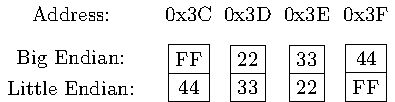
\includegraphics[width=0.8\textwidth]{endian}
						\caption{Big and little endian representation}
						\label{fig:endian}
					\end{figure}	
			\end{enumerate}
		\item Convert the following MIPS assembly code into machine language. Write
			the instructions in hexadecimal.\\
			\texttt{add \$t0, \$s0, \$s1}\\
			opcode: 0, rs: 16, rt: 17, rd: 8, shamt: 0, funct: 32\\
			000000 10000 10001 01000 00000 100000\\
			$0000|0010|0001|0001|0100|0000|0010|0000 \to$ \textbf{0x02114020}\\
			\texttt{lw \$t0, 0x20(\$t2)}\\
			opcode: 35, rs: 10, rt: 8, imm: 32\\
			100011 01010 01000 0000000000010000\\
			$1000|1101|0100|1000|0000|0000|0001|0000 \to$ \textbf{0x8D480010}\\
			\texttt{addi \$s0, \$0, -10}\\
			opcode: 8, rs: 0, rt: 16, imm: -10\\
			001000 00000 10000 1111111111110110\\
			$0010|0000|0001|0000|1111|1111|1111|0110 \to$ \textbf{0x2010FFF6}
		\pagebreak
		\item The \texttt{nori} instruction is not part of the MIPS instruction set,
			because the same functionality can be implemented using existing instructions.
			write a short assembly code snippet that has the following functionality:
			\texttt{\$t0 = \$t1 NOR 0xF234}. Use as few instructions as possible.\\
			\texttt{ori \$t0, \$t1, 0xF234\\
				nor \$t0, \$t0, \$0}\\
		\item Implement the following high-level code segments using the \texttt{slt}
			instruction. Assume the integer variables \texttt{g} and \texttt{h} are
			in registers \texttt{\$s0} and \texttt{\$s1} respectively.\\
			\texttt{if(g $\le$  h) \{g = 0;\}\\
			else \{h = 0;\}}\\\\
			\texttt{slt \$t0, \$s1, \$s0\ \ \ \ \# if(g $\le$ h)\\
				beqz \$t0, label1\ \ \ \ \ \# g is $\le$ h\\
                                addi \$s1, \$0, 0\ \ \ \ \ \ \# h = 0\\
                                j end\ \ \ \ \ \ \ \ \ \ \ \ \ \ \ \ \# finish program\\
				label1:\\
				addi \$s0, \$0, 0\ \ \ \ \ \ \# g = 0\\
				j end\ \ \ \ \ \ \ \ \ \ \ \ \ \ \ \ \# skip else statement\\}
				
	\end{enumerate}
\end{document}
